\section{Messing with MOSFETs}
\label{lab_mosfet}

%\makelabheader %(Space for student name, etc., defined in master.tex)

\bigskip

A \textit{MOSFET} (short for \textit{metal-oxide-semiconductor field-effect transistor}) is in many ways an improvement on the JFET.  The MOSFET's low channel resistance allows it to handle large currents, and its electrically insulated gate allows gate voltages $V_\text{GS}$ that are the same polarity as $V_\text{DS}$.  Both of these make MOSFETs ideal for simple circuits that switch large currents on and off.

\bigskip
\textbf{A Pulse-Width Modulation (PWM) Controller}
\begin{enumerate}[wide]
\item The circuit below shows a standard square wave generator made using a 555 timer in astable mode, just as you did in Lab~\ref{lab_timers}.  An additional resistor $R_\text{lim}$ has been added in series with $R_1$ to protect against the DISCH lead being connected directly to $V\text{CC}$.  Build the circuit as shown below, but replace $R_1$ and $R_2$ with your PB-505's $10\kohm$ potentiometer and a diode, so that you can adjust the duty cycle from $\approx 0\%$ (potentiometer full counterclockwise) to  $\approx 100\%$ (full clockwise).  Choose $C$ such that at a duty cycle of $\approx 50\%$, $f\approx 50$~Hz.  
\label{part_variable_duty_astable}
\begin{center}

\includegraphics{mosfet/astable_555.pdf}
\end{center}

\item The small DC motor in you kit requires a voltage between $\approx$1~VDC and 6~VDC, but it draws a large current of up to $\approx$1~A or more.  Set your variable voltage supply $+V$ to 3~V, and use your multimeter to measure the current drawn by the motor.  Does slowing the motor with your fingers affect the current?  Explain your findings, using the key words \textit{inductance}, \textit{resistance}, and \textit{commutator}---the latter of which Google will be happy to tell you all about.

\figuretoright{0.25}[scale=0.8]{mosfet/mosfet_motor.pdf}{
\item The circuit to the right shows a transistor controlling a load such as a DC motor.  From the diagram, what type of transistor is the HUF76423p3?  (JFET or MOSFET? N-channel or p-channel?  Enhancement mode or depletion mode?)
\smallskip

\item Build the circuit to the right using your variable duty-cycle generator from part~\ref{part_variable_duty_astable} as the control voltage $V_\text{in}$, and your DC motor as the load.  Are you able to control the speed of your motor this way?  This arrangement is called a \textit{Pulse Width Modulation} or \textit{PWM} controller---that is, you are \textit{modulating} the pulse width to control the power to the motor.  On a scale from 1 to 10, how emotionally satisfying is this? 
}

\item An arguably simpler strategy for controlling the power to your DC motor would be to use a bipolor junction transistor, connecting the motor to either the emitter or collector and applying an adjustable \textit{DC voltage} to the transistor's base---no 555 timer required at all.  What would be the main disadvantage of that method compared to the PWM controller? (Hint: consider consulting either Linda or Swintayla from problem~\ref{prob_Linda_Swintayla}.)

\pagebreak[3]
\textbf{Measuring the HUF76423p3 transistor}

\item Use the $1\kohm$ potentiometer on your PB-505 to vary the output voltage of your pulse generator from 0~V (full counterclockwise) to 5~V (full clockwise) as in the circuit below. 
Monitor your circuit with the first three channels of your friend the oscilloscope at the places shown.  You will notice that the measurement of Ch~3 is noisy as heck.  Why is this?  (Hint: does the noise change if you slow the motor with your fingers?) 

\begin{center}
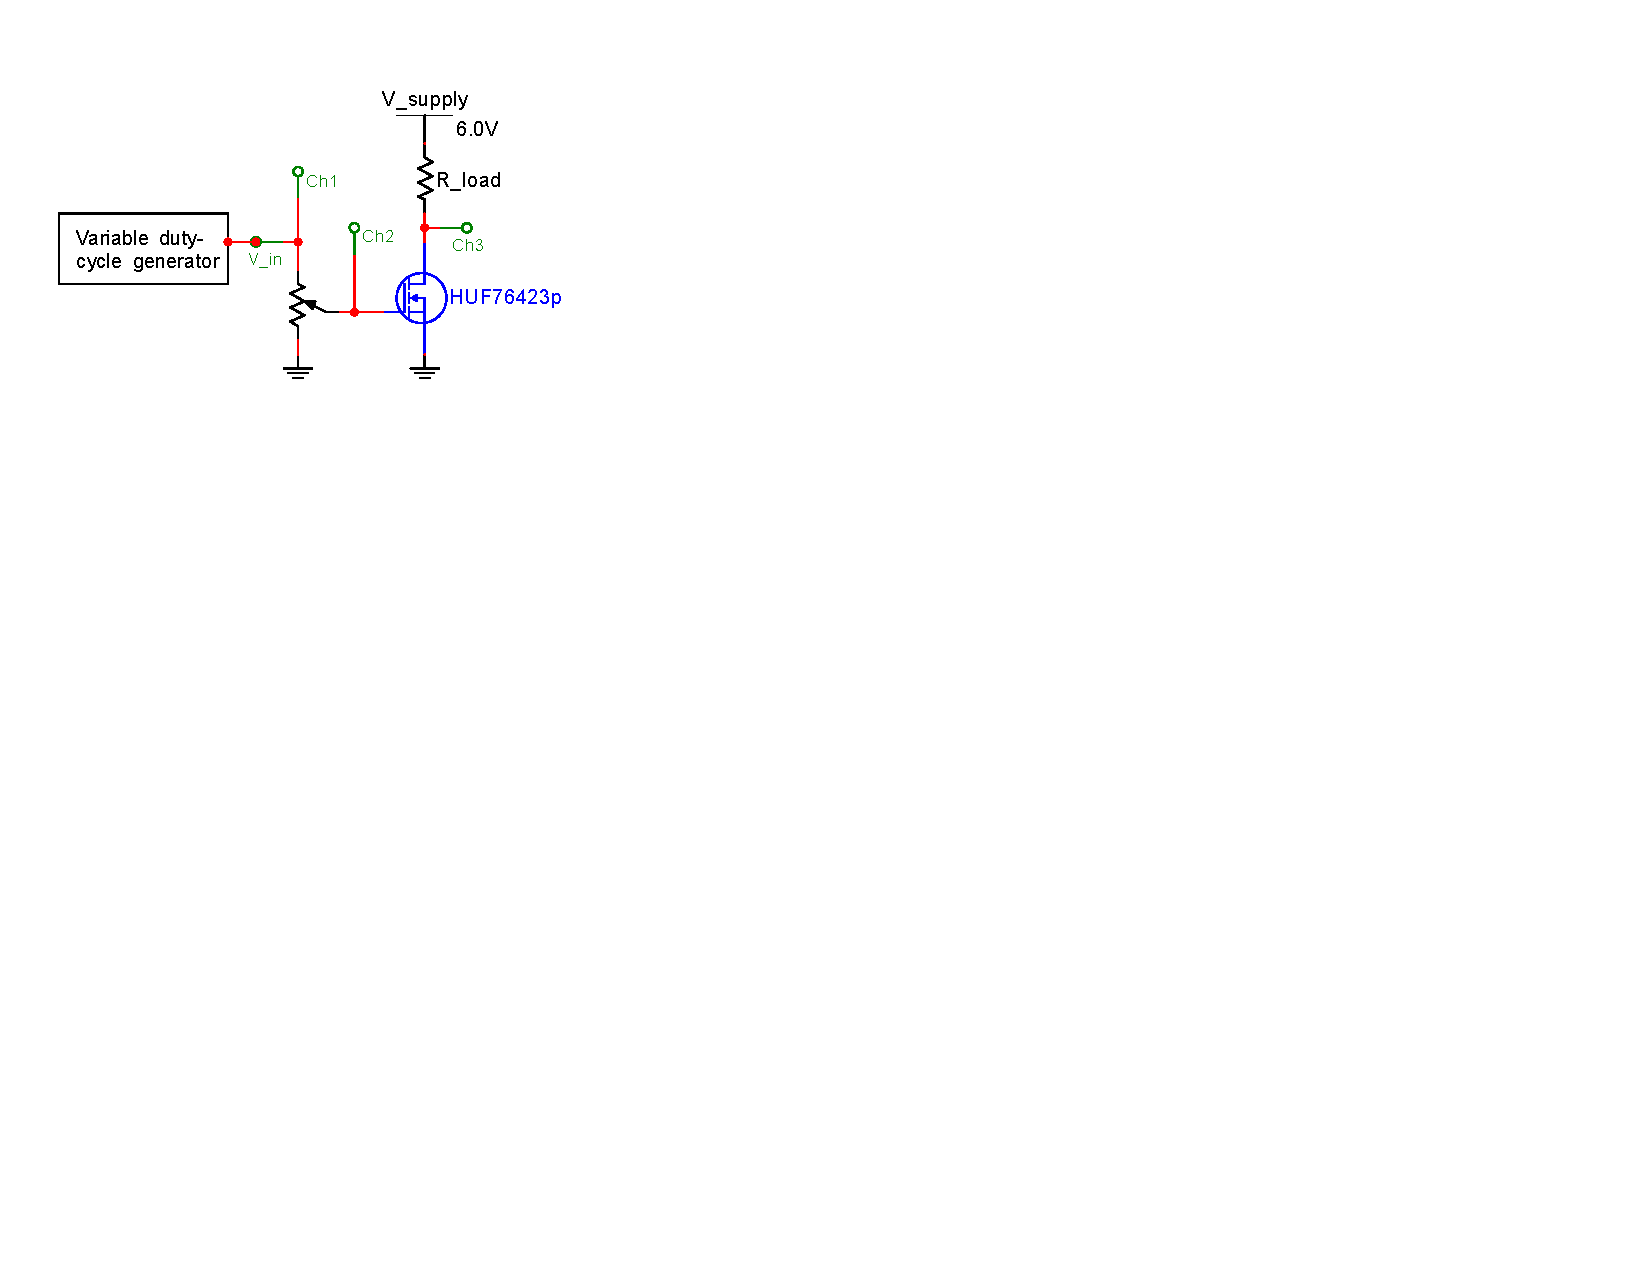
\includegraphics{mosfet/mosfet_motor_2pots.pdf}
\end{center}


\item To eliminate the noise from the DC motor, we'll switch the load to a 1~W, $10\ohm$ load resistor.  At this point, we'll want to be careful not to overheat either the MOSFET or the load resistor, so we'll set the duty cycle of the PWM to $\approx 5\%$ or below.  This is a common trick used in electrical testing: using short duty cycles to allow high currents and voltages that would otherwise damage the component being tested.

With $V_\text{GS}=5$~V ($1\kohm$ pot full clockwise) and $V_\text{supply}=10$~V,  what is $V_\text{DS}$?  What is the apparent channel ``resistance'' under these conditions? 
Note: because the $I$-$V$ characteristics of the channel are highly nonlinear, the ``resistance'' (note the scare quotes) is often denoted with a lower-case letter as $r_\text{DS}$.
\label{part_r_DS}

\item We can also measure current by inserting an additional \textit{current sensing} resistor $R_\text{curr} = 0.1\ohm$ in series with the channel and the load. Build the circuit below and confirm that the your measured $r_\text{DS}$ from part~\ref{part_r_DS} is correct.

\begin{center}
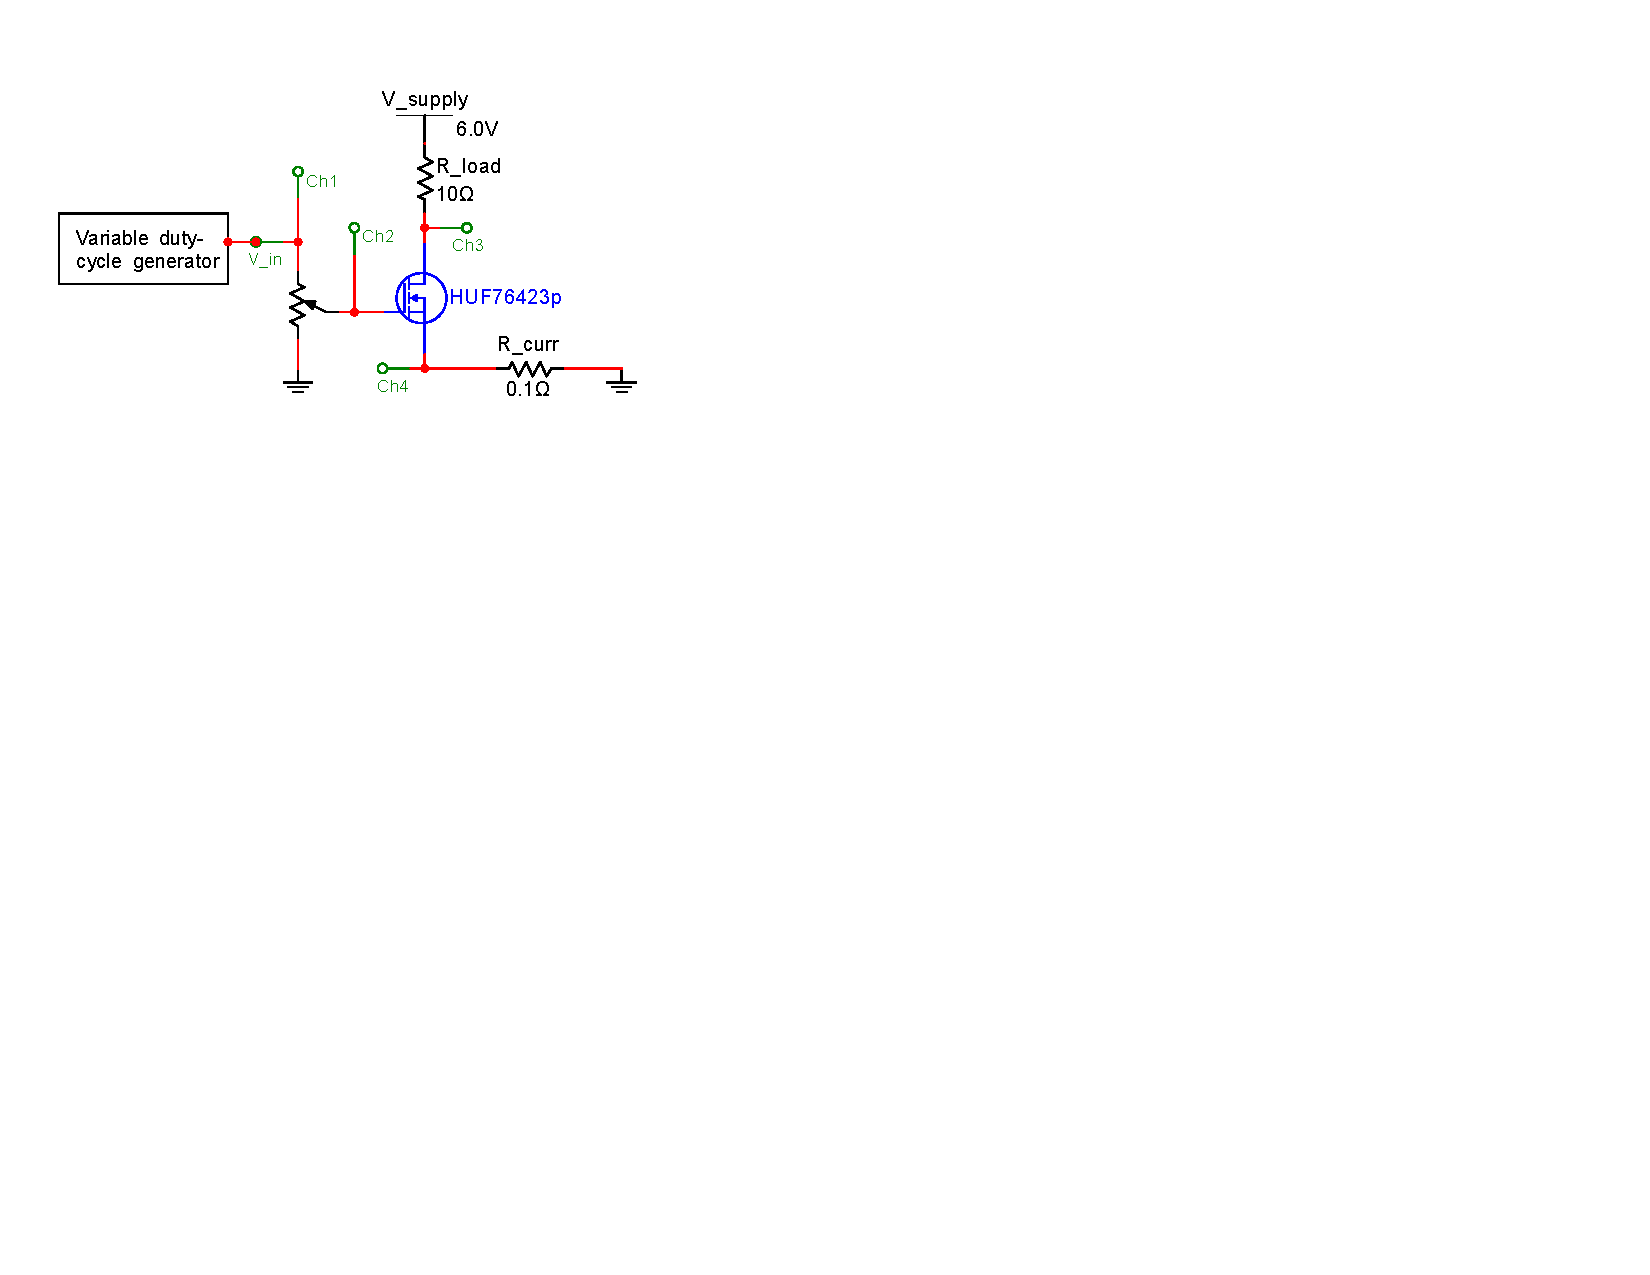
\includegraphics{mosfet/mosfet_motor_4chan.pdf}
\end{center}



\item Use the $10\kohm$ pot to adjust $V_\text{GS}$.  At what voltage $V_\text{GS}$ does $I_\text{DS}$ begin to rise?  At what $V_\text{GS}$ does $I_\text{DS}$ reach its maximum?  Are your measurements consistent with the \textit{threshhold voltage} $V_\text{GS(TH)}$ in the datasheet?



\end{enumerate}








